\chapter{Аналитический раздел}
\label{cha:analysis}

Для решения поставленных задач необходимо чётко формализовать, чем является спиральная галактика, какими свойствами, поведением она обладает, из чего состоит.

\section{Структура и типы галактик}

Галактика представляет собой гравитационно-связанную систему объектов и множеств объектов таких, как звёзды, звёздные скопления, планеты и так далее. Данное понятие само по себе абстрактно, поэтому необходимо представить классификацию галактик для конкретизации задания.

Заметно большие отличия между различными галактиками видны даже при поверхностном анализе их фотографий. По внешнему виду галактики делятся на неправильные, линзовидные, эллиптические и спиральные\cite{konon}. Данная курсовая работа посвящена последнему типу.

Структура спиральных галактик характерна наличием спиральных ветвей. Эти ветви выделяются на общем фоне диска за счёт высокой светимости и высокой плотности объектов внутри. Все спиральные галактики имеют схожее строение, в основе которого можно выделить три составляющих: звёздный диск, сфероидальная составляющая, плоская составляющая. Толщина звёздного диска в пять-десять раз меньше диаметра самой галактики. Толщина же плоской составляющей галактики меньше толщины звёздного диска в несколько раз. Балдж — это яркая область внутри сфероидальной составляющей галактики. В самом центре находится ядро. Спиральные галактики обозначаются литерой S\cite{konon}.

Во многих спиральных галактиках во внутренней области звёздами образуется так называемый бар — вытянутая перемычка. От концов бара отходят спиральные ветви. Примером такой галактики является наша, Млечный Путь. Спиральные галактики с баром обозначаются литерами SB.

По виду спиральной структуры галактики выделяют следующие подтипы:
\begin{itemize}
    \item галактики с туго закрученными спиральными ветвями. К обозначению данного подтипа галактик в конец добавляется литера a;
    \item галактики с широко раскрытыми спиральными ветвями. В зависимости от особенностей строения таких галактик к их обозначению добавляется либо литера c, либо литера d;
    \item галактики, обладающие промежуточными свойствами описанных выше подтипов. К их обозначению добавляется литера b.
\end{itemize}
Для упрощения решения задачи моделирования, далее под спиральными галактиками будут подразумеваться галактики типа Sa.

Даже внутри одного типа галактики имеют серьёзные визуальные отличия друг от друга. Это обусловлено различием их параметров. Перечислим их:
\begin{itemize}
    \item радиус ядра;
    \item радиус диска;
    \item количество составных объектов;
    \item скорость вращения спиральных рукавов;
    \item температуры составных объектов.
\end{itemize}

На основе проделанного анализа можем выявить подзадачи, которые необходимо решить, чтобы добиться реалистической модели спиральной галактики:
\begin{itemize}
    \item определение состава галактики;
    \item распределение объектов системы в пространстве;
    \item определение принципов движения объектов галактики;
    \item вычисление характеристик составных частей галактики: скорость, температура.
\end{itemize}

\section{Формализация объектов сцены}

Состав спиральной галактики разнообразен, в него входят звёзды, планеты, шаровые скопления, звёздная пыль и так далее. Очевидно, эти объекты имеют серьёзные различия как в контексте визуализации, так и в контексте моделирования. Но так же существует и то, что их объединяет. Например - Первый закон Кеплера: каждая планета Солнечной Системы обращается по эллипсу, в одном из фокусов которого находится Солнце. Этот закон был подобран эмпирически, а его обобщение применимо не только к звёздным системам, но и к галактикам, где на роль планет приходят объекты галактики, а на место Солнца - её центр.

Так как поведенческий аспект составных частей звездной системы приблизительно совпадает, то в ущерб визуальной составляющей ограничим состав формируемой модели только звёздами. Такое решение обусловлено тем, что визуализация именно таких небесных тел или систем тел, как шаровые скопления, звёздная пыль, является отдельной, требующей глубокого анализа, темой.

Важно отметить, что каждая звезда является источником света. Но в контексте данной работы реализация модели освещения для сцены не влияет на реалистичность итогового изображения, но при этом требует использование аппаратных ресурсов, поэтому было принято решение не осуществлять её.

Говорить о относительно чётком значении количества звёзд в галактике довольно тяжело. По современным оценкам Млечный Путь насчитывает 200-400 миллиардов звёзд, Туманность Андромеды — около 1 триллиона. Даже карликовые галактики насчитывают несколько миллиардов звёзд. Безусловно, система частиц из столь большого количества элементов требует колоссальных аппаратных ресурсов для обработки. Кроме того, никакое ныне поддерживаемое разрешение экрана не способно отобразить такое огромное количество элементов. А ведь помимо звёзд в состав галактик входят многие другие объекты, такие как планеты, их спутники. Очевидно, что требуется упрощение, жертвующее детализацией и реалистичностью в угоду производительности. Таким упрощением может послужить система частиц, состоящая из элементов, количество которых лежит на отрезке $[1\cdot{}10^2, 3\cdot{}10^4]$.

\subsection{Система частиц}

Так как галактика по своей природе не имеет чётких границ и по определению является системой космических объектов, целесообразно использовать для её виртуального представления систему частиц. Система частиц состоит из определённого некоторым образом количества частиц, математически представляемых как материальные точки. Для абстрактной частицы этой системы выделяются атрибуты, например:
\begin{itemize}
	\item положение в пространстве;
	\item скорость;
	\item внешний вид;
	\item время жизни
\end{itemize}

Для любой частицы системы существует единый закон, определяющий принципы и модель поведения этой частицы. Общепринятых способов визуализации, как и многих других аспектов реализации системы частиц, нет. Использование системы частиц предполагает, что кол-во этих самых частиц в системе велико. Данная особенность означает, что применение к системе частиц методов, требующих трудоёмкие или ресурсоёмкие вычисления, влечёт за собой огромные потери во времени или в памяти соответственно. Поэтому для системы частиц существует ряд упрощений. Например, частицы не поглощают свет и не отбрасывают тень.

\section{Анализ теорий движения звёзд}
Рассматриваемый тип галактик имеет нетривиальный динамический спиральный узор. Чтобы воссоздать его, необходимо определить, каковы траектории движения звёзд.

Обратим внимание на структуру узора спиральных галактик и её особенности. На по большей части тусклом диске выделяются яркие линии — спиральные рукава. Этот факт можно объяснить разными способами.

Во-первых, молодые звёзды излучают свет большей интенсивности, чем старые звёзды. Значит, в состав спиральных ветвей входят по большей части молодые звёзды, выделяя таким образом их на общем узоре галактического диска.

Во-вторых, повышенная яркость спиральных рукавов может объясняться повышенной кучностью входящих в их состав звёзд.

Для реалистичной имитации спиральной галактики необходимо определить природу спиральных рукавов, и как их наличие сказывается на закон, определяющий движение звёзд в галактике.

\subsection{Дифференциальное вращение}

Как было сказано ранее, Первый закон Кеплера применим к галактикам. То есть, каждая звезда в галактике движется по эллипсу, в фокусе которого находится центр этой галактики.

Чтобы определить, какую роль в этом движении занимают спиральные ветви, нужно обозначить их природу. Допустим, что спиральные рукава имеют материальную природу, то есть помимо звёзд они состоят из какого-то вещества.

Если это вещество имеет жидкую или газообразную структуру, то галактика вращается дифференциально, то есть различные её составляющие имеют различную угловую скорость. Но у данной идеи есть явный недостаток: при дифференциальном вращении вследствие нескольких оборотов спиральные рукава галактики превратятся в очень туго закрученные, несмотря на свою начальное состояние. Таким образом, структура галактики будет нарушена, что есть противоречие.

\subsection{Твердотельное вращение}
Чтобы поддерживать спиральный узор, вещество, образующее ветви, должно иметь устойчивую структуру, а значит спиральные ветви вращаются твердотельно. В этом случае происходит визуальное несоответствие с действительностью — спиральные рукава не только устойчивы в своей структуре, но и в пространстве. Несмотря на то, что звёзды в галактике движутся, спиральные ветви не меняют своего положения относительно центра галактики. Следовательно, данное предположение о природе спиральных ветвей так же ложно.

\subsection{Теория волн плотности}
Усложнение материальной природы спиральных ветвей неуместно, так как это может повлиять на остальные законы поведения космических тел. Следовательно, справедливо предположение, что природа спиральных рукавов нематериальна.

К такому же выводу пришли американские учёные китайского происхождения Цзя-цзяо Линь и Фрэнк Шу. По их мнению, спиральные ветви — это области повышенной звёздной плотности. Можно привести известный и наглядный пример с движением автомобилей на дорогах: в какой-то момент времени машины движутся свободно, их кучность мала, но иногда образуется автомобильный затор, который впоследствии сходит на нет и транспорт снова движется свободно. То есть спиральные рукава — это такие же «пробки».

Более формальное определение спиральных ветвей согласно вышеописанной теории обозначает их как долгоживущие квазистационарные волны повышенной плотности, находящиеся на звёздном диске галактики.

Таким образом, мы получаем модель, которая обеспечивает достаточно постоянную структуру спиральных ветвей, так как траектории движения звёзд в галактике устойчивы.

Как было сказано ранее, каждая звезда движется по эллипсу, в фокусе каждого из этих эллипсов находится центр галактики. Теория волн плотности позволяет сделать вывод о том, что эти эллипсы имеют последовательную взаимосвязь. Чтобы области повышенной плотности на галактическом диске были возможны, нужно, чтобы каждая следующая траектория-эллипс была повёрнута относительно предыдущей на некоторый переменный угол. Пример такой картины можно увидеть на рисунке \ref{img:densitywaves}.

\begin{figure}[H]
    \centering
	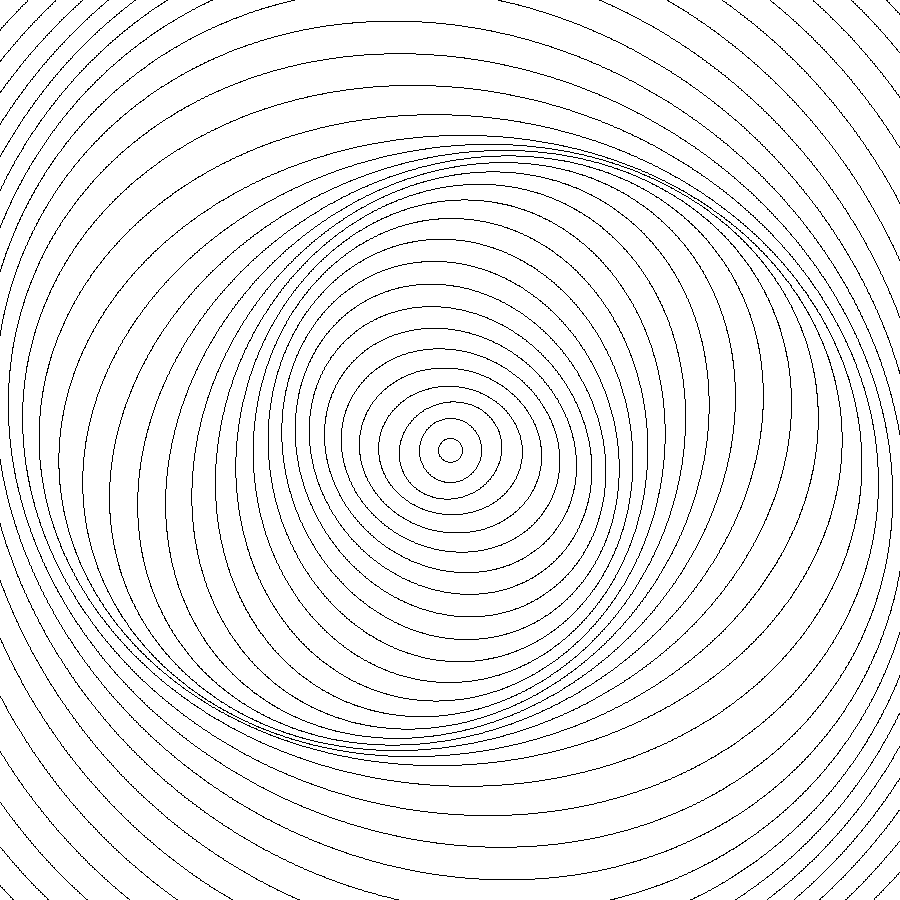
\includegraphics[scale=0.4]{image/densitywaves.png}
	\caption{Волны плотности}
	\label{img:densitywaves}
\end{figure}

Тут отчётливо видны области повышенной плотности, другими словами, спиральные ветви.

\subsection{Вывод}

Как итог, единственный способ создать реалистическую модель спиральной галактики — это использование теории волн плотности при вычислении траекторий движений звёзд. Все остальные способы не подходят.

\section{Анализ способов распределения звёзд в пространстве}

Распределение звёзд в пространстве можно разбить на два этапа: размещение в плоскости диска и размещение по вертикали.

\subsection{Плоскость диска}

Плотность звёзд на поверхности диска галактики уменьшается с увеличением расстояния до её центра. Для того, чтобы разместить звёзды в пространстве, необходимо знать функцию распределения вероятности, где случайной величиной является расстояние до центра галактики. В этом случае можно было бы прибегнуть к уже известным законам распределения, но лучше обратиться к закону распределения, связанному с физикой самой галактики.

Концентрация звёзд на некотором участке влияет на испускаемую на этом участке светимость. Так же существует закон де Вокулёра, изображающий зависимость поверхностной яркости эллиптической галактики от видимого расстояния до его центра:
\begin{equation}
	I(R) = I_0 \cdot{} e^{-k\cdot{}R^\frac{1}{4}}
\end{equation}
здесь $I$ - поверхностная яркость, $I_0$ - значение поверхностной яркости в центре галактики, $R$ - расстояние до центра, $k$ - эмпирически подбираемая константа, которая может быть равна, например, 0.02.

Особенность ядра спиральной галактики заключается в том, что яркость на его поверхности имеет приблизительно такую же зависимость от $R$, как и яркость на поверхности эллиптической галактике. Существует так же обобщение закона де Вокулёра для галактик разных типов, закон Серсика:
\begin{equation}
	I(R) = I_0 \cdot{} e^{-v_n(\frac{R}{R_0})^\frac{1}{n}}
\end{equation}
тут $n$ - параметр, являющийся натуральным числом и определяющий тип галактики. Для диска спиральной галактики $n = 1$. Значение $v_n$ подбирается так, чтобы в пределах $R_0$ излучалась половина всей светимости галактики, $v_1 = 1.67834699$.

Таким образом можем записать функцию поверхностной яркости от расстояния до центра галактики:
\begin{equation}
    I(R) = \left\{ \begin{array}{ll}
		I_0 \cdot{} e^{-k\cdot{}R^\frac{1}{4}}, 		& \textrm{$R \leq{} R_c$}\\
		I_0 \cdot{} e^{-v_n(\frac{R}{R_0})^\frac{1}{n}} & \textrm{Иначе}\\
	               \end{array} \right.
\end{equation}
где $R_c$ - радиус ядра галактики.

Полученная функция является убывающий, в то время как функция распределения вероятностей - неубывающая. Тогда пусть - $F_I(x)$ - интересующая нас функция распределения, так же $R_{min}$, $R_{max}$ - минимальное и максимальное расстояния от центра галактики, где могут быть звёзды, и:
\begin{equation} \label{eq:F_I}
	F_I(x) = \left\{ \begin{array}{ll}
		0, & \textrm{$x \leq{} R_{min}$}\\
		\frac{\int_{R_{min}}^x I(t)dt}{\int_{R_{min}}^{R_{max}} I(t)dt}, & \textrm{$R_{min} < x \leq{} R_{max}$}\\
		1, & \textrm{$x > R_{max}$}\\
			 \end{array} \right.
\end{equation}

Полученную функцию распределения вероятностей можно использовать для размещения звёзд в плоскости диска спиральной галактики.

\subsection{Вертикальная составляющая}

Так как диск спиральной галактики имеет форму приближенную к окружности, то на любой плоскости, перпендикулярной плоскости диска, проекция звёзд будет очерчивать приблизительно одну и ту же форму - форму эллипса, у которого одна полуось в 5-10 раз больше другой. На рисунке \ref{img:miklyway} изображён пример в виде Млечного Пути.

\begin{figure}[H]
    \centering
	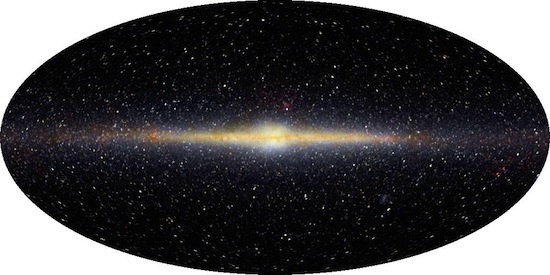
\includegraphics[scale=0.4]{image/MilkyWay.jpg}
	\caption{Инфракрасное изображение Млечного Пути}
	\label{img:miklyway}
\end{figure}
Здесь чётко видно, что, чем больше расстояние до плоскости диска, проходящей через центр галактики, тем меньше плотность звёзд. Чтобы добиться такого эффекта необходимо воспользоваться некоторым законом распределения, где случайной величиной является только что упомянутое расстояние.

Наиболее подходящим таким законом является нормальное распределение. Распределение Гаусса очень часто встречается в природе (характеристики и модели поведения живых организмов, статистические наблюдения, отклонение при стрельбе и многие другие ситуации), благодаря чему и получило название "нормальное".

\section{Кривая вращения галактики}
Скорость вращения звезды вычисляется по формуле:
\begin{equation}
	v(r) = \sqrt{r \cdot{} \frac{d\Phi{}(r)}{dr}}
\end{equation}
где $r$ - расстояние до центра галактики, $\Phi{}$ - гравитационный потенциал:
\begin{equation}
	\Phi{}(r) = -\frac{GM(r)}{r}
\end{equation}
тут $G$ - гравитационная постоянная, M - точечная масса, расположенная в центре системы. Спиральная галактика - сложная система. Если учитывать влияние только звёзд, такая масса равна:
\begin{equation}
	M_{sg}(r) = \rho{}_{sg}(r) \cdot{} V_{sg}(r) = \rho_{sg0} \cdot{} e^{-\frac{r}{R_h}} \cdot{} V_{sg}(r)
\end{equation}
где $\rho{}_{sg}(r)$ - плотность звёзд на расстоянии $r$ от центра, $\rho{}_{sg0} = \rho{}_{sg}(0)$, $V_{sg}(r)$ - объём, охватываемый галактикой на расстоянии $r$.

Существует проблема вращения галактик - массы видимой массы галактики не достаточно для достижения звёздами наблюдаемой скорости. Поэтому в наше время считается, что в галактике присутствует некая невидимая тёмная материя, имеющая массу:
\begin{equation}
	M_{dm}(r) = \rho{}_{dm}(r) \cdot{} V_{dm}(r)
\end{equation}
где $\rho{}_{dm}$ плотность тёмной материи:
\begin{equation}
	\rho{}_{dm}(r) = \rho{}_{dm0} \cdot{} (1 + (\frac{r}{R_c})^2)^{-1}
\end{equation}
$\rho{}_{dm0}$ - плотность тёмной материи в центре системы, $V_{dm}$ - объём гало, сферической оболочки, тёмной материи в галактике.

Тогда имеем формулу:
\begin{equation}
	M(r) = M_{sg}(r) + M_{dm}(r)
\end{equation}

\section{Окрашивание звёзд}
Цвет звезды зависит от её температуры, которая меняется на протяжении всей её жизни. Так как в разрабатываемой системе частиц время жизни частицы не ограниченно её внутренними свойствами, справедливо допущение, при котором температура отдельно взятой звезды постоянна.

Чтобы получить цветовой спектр излучения звезды в соответствии с её температурой, необходимо обратиться к закону Планка. Результат изображён на рисунке \ref{img:spectrum}.
\begin{figure}[H]
    \centering
	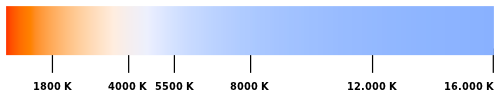
\includegraphics[scale=0.6]{image/spectrum.png}
	\caption{Цветовой спектр температур в соответствии с законом Планка}
	\label{img:spectrum}
\end{figure}

\section{Синтез изображения}
С точки зрения визуализации поставленная задача состоит в рисовании точечных объектов системы частиц. Применение алгоритмов удаления невидимых линий и поверхностей, закрашивания нецелесообразно. Таким образом, синтез изображения сводится к следующим шагам:
\begin{enumerate}
	\item разработка трёхмерной математической модели синтезируемой визуальной обстановки;
	\item задание положения наблюдателя, картинной плоскости, размеров окна вывода;
 	\item преобразование координат объектов в координаты наблюдателя;
	\item отсечение объектов по границам пирамиды отсечения;
	\item вычисление двумерных перспективных проекций объектов сцены на картинную плоскость;
	\item вывод полученного изображения на экран.
\end{enumerate}

\subsection{Координаты наблюдателя}

Наблюдатель задаётся тремя векторами:
\begin{itemize}
	\item $\vec{A}$ - положение наблюдателя;
	\item $\vec{B}$ - точка, в которую обращён взгляд наблюдателя;
	\item $\vec{C}$ - нормированная нормаль, указывающая, где верх камеры.
\end{itemize}
На основе этих векторов получим:
\begin{equation}
	\vec{D} = \vec{A} - \vec{B}
\end{equation}
\begin{equation}
	\vec{E} = \vec{C} \times{} \vec{D}
\end{equation}
\begin{equation}
	\vec{E_n} = \frac{\vec{E}}{|\vec{E}|}
\end{equation}

Тогда, чтобы перейти к координатам наблюдателя, необходимо все точки системы умножить на матрицу:

\begin{equation}
	\begin{bmatrix}
		\vec{E_n}.x && \vec{E_n}.y && \vec{E_n}.z && 0 \\
		\vec{C}.x  &&  \vec{C}.y  &&  \vec{C}.z  &&  0 \\
		\vec{D}.x  &&  \vec{D}.y  &&  \vec{D}.z  &&  0 \\
		\vec{A}.x  &&  \vec{A}.y  &&  \vec{A}.z  &&  1
	\end{bmatrix}
\end{equation}

Для перемещения наблюдателя в пространстве сцены необходимо использовать аффинные преобразования относительно центра галактики.

\subsection{Пирамида отсечения}

Пусть $\alpha{}$ - угол обзора (в радианах), $k$ - соотношение сторон экрана, $n$ - расстояние до ближней плоскости отсечения, $f$ - расстояние до дальней плоскость отсечения. Умножая координаты объектов системы на матрицу:

\begin{equation}
	\begin{bmatrix}
		\frac{2}{k \cdot{} tg(\alpha{})} && 0 && 0 && 0 \\
		0 && \frac{2}{tg(\alpha{})} && 0 && 0 \\
		0 && 0 && -\frac{f + n}{f - n} && -1 \\
		0 && 0 && -2\cdot{}\frac{f\cdot{}n}{f - n} && 0
	\end{bmatrix}
\end{equation}
можно получить однородные координаты, в которых достаточно просто отсечь точки по границам пирамиды отсечения: точки, у которых значение хотя бы одной координаты $\notin [-w, w]$, отбрасываются. $w$ - это последняя компонента вектора в однородных координатах.

\section{Вывод}
Анализ физических законов и алгоритмов синтеза сложных динамических изображений закладывает основы в разработке реалистической модели спиральной галактики и её визуализации.

